\documentclass[12pt]{article}
\usepackage{tikz}
\usepackage{amsmath}
\usepackage{amssymb}
\usepackage{float}
\usepackage{caption}
\usepackage{array}
\usepackage{cancel}
\usepackage{longtable}

\title{\textbf{Logarithms Course}\\
\begin{center}
\includegraphics[width=4em]{ApS_logo.png}
\end{center}
\begin{normalsize}Applied Scholastics, Ferndale \end{normalsize}}
\author{}
\date{}

\begin{document}
\maketitle

\section*{Logarithms}

\subsection*{History \& Purpose}

A logarithm is the power to which a base number must be raised to equal a given number.\\
The base is written as a subscript next to the word ‘log.’
\begin{Large}
\begin{align*}
number &= base^{power}\\
log_{base} number &= power
\end{align*}
\end{Large}
$$\text{(Given }base>0, base\neq1\text{, and }number>0.)$$
For example, for a base of $10$, since $100 = 10^2$, the logarithm of $100$ is $2$.
  $$100=10^2\text{ so }\log_{10}100=2$$

\begin{enumerate}

\item What is a logarithm?
\item For a base of 10, what is the logarithm of 1000?
\item How do you write this?
\item For a base of 2, what is the logarithm of 16?
\item How do you write this?

Logarithms were developed in the 1600s by mathematicians John Napier and John Briggs. The word was coined by Napier from the Latin words logos and arithmos and means ‘ratio-number.’\\

With scientific advances in fields such as astronomy, navigation, time keeping and map making, it had become necessary to perform more and more long and tedious calculations with large numbers by hand. Logarithms were invented to make working with large numbers easier and faster.\\

\item Why were logarithms invented?

Napier used a base of $e$ for his logarithms. This is ‘Euler’s number,’ roughly equal to 2.7183. Euler was a famous mathematician and $e$ was named after him. It is a constant that often turns up in studies of the natural world and it is used in many branches of mathematics. It was first discovered in solving a problem to do with compound interest. Logarithms with a base of $e$ are called natural logarithms and are written as $\ln n$ or $\log_e n$.\\

Briggs later introduced the base of 10 as being easier to work with decimal numbers. Logarithms with a base of 10 are called common logarithms and are written simply as $\log n$ without indicating the base. You can assume that the base of a logarithm is 10 unless it is indicated otherwise.

\begin{center}
e.g.
\begin{tabular}{ l l }
$\log{25}=\log_{10}25\approx1.3979$ & $10^{1.3979}\approx25$\\
$\ln 25=\log_{e}25\approx3.2189$ & $e^{3.2189}\approx25$\\
\end{tabular}
\end{center}

\begin{center}
e.g.
\begin{tabular}{ l l }
$16 = 4^2$ & $\log_4{16}=2$\\
$4 = 8^{\frac{2}{3}}$ & $\log_8{4}=\frac{2}{3}$\\
$1000 = 10^3$ & $\log{1000}=3$
\end{tabular}
\end{center}

\item What is Euler's number?
\item What are logarithms with a base of $e$ called?
\item How are natural logarithms written?
\item What are common logarithms?
\item Why was a base of 10 preferred?
\item What base is assumed in $\log25$?

Tables were calculated where the logarithm of any number could be easily looked up. The product of two numbers could be found simply by looking up their logarithms, adding these logarithms, and then looking in the table for the antilogarithm, which meant the number with that logarithm.\\

Similarly, any two numbers could be quickly divided by taking the difference of their logarithms and looking up that antilogarithm as their quotient.\\

Lengthy problems in multiplication and division were changed by use of logarithms to simple problems of addition and subtraction.\\

\begin{center}
\includegraphics[width=0.8\textwidth]{log table sample.png}\\
Part of a table from a book of logarithms\\
\end{center}

For example, 123 and 234 can be multiplied by looking up their logarithms ($2.09$ and $2.37$), adding them together ($2.09+2.37=4.46$), and looking through the values of the table to find the number that has that logarithm, the antilogarithm.\\
\begin{align*}
\log_{10}123&=2.09\\
\log_{10}234&=2.37\\
2.09+2.37&=4.46\\
\log {28,782}&=4.46\\
\text{so, }123 \times 234&=28,782\\
\end{align*}

\item How is multiplication done with logarithms?
\item Given that $\log456=2.5690$ and $\log567=2.7536$, and that the antilog of $2.5690+2.7536=5.4125$ is $258524$, what is $456\times567$?

\vspace{12pt}
That's the basic idea, but the real power of logarithms comes from their use with larger numbers.\\

To demonstrate the amount of work that is saved by using logarithms, here is an example of multiplying two long numbers by hand, calculating partial products for each digit of the multiplier multiplied by each digit of the multiplicand, and then adding all of the partial products. Multiplying like this can made shorter by "carrying" digits and so on, but even with that it is still long, tedious and error-prone.

\begin{center}
\begin{longtable}
{c@{\,}c@{\,}c@{\,}c@{\,}c@{\,}c@{\,}c@{\,}c@{\,}c@{\,}c@{\,}c@{\,}c}
 & & & &      & &1&2&3&4&5&6\\
 & & & &\times& &2&3&4&5&6&7\\
\hline 
 & & & & & & & & & &4&2\\
 & & & & & & & & &3&5& \\
 & & & & & & & &2&8& & \\
 & & & & & & &2&1& & & \\
 & & & & & &1&4& & & & \\
 & & & & & &7& & & & & \\
 & & & & & & & & &3&6& \\
 & & & & & & & &3&0& & \\
 & & & & & & &2&4& & & \\
 & & & & & &1&8& & & & \\
 & & & & &1&2& & & & & \\
 & & & & &6& & & & & & \\
 & & & & & & & &3&0& & \\
 & & & & & & &2&5& & & \\
 & & & & & &2&0& & & & \\
 & & & & &1&5& & & & & \\
 & & & &1&0& & & & & & \\
 & & & &5& & & & & & & \\
 & & & & & & &2&4& & & \\
 & & & & & &2&0& & & & \\
 & & & & &1&6& & & & & \\
 & & & &1&2& & & & & & \\
 & & & &8& & & & & & & \\
 & & &4& & & & & & & & \\
 & & & & & &1&8& & & & \\
 & & & & &1&5& & & & & \\
 & & & &1&2& & & & & & \\
 & & & &9& & & & & & & \\
 & & &6& & & & & & & & \\
 & &3& & & & & & & & & \\
 & & & & &1&2& & & & & \\
 & & & &1&0& & & & & & \\
 & & & &8& & & & & & & \\
 & & &6& & & & & & & & \\
 & &4& & & & & & & & & \\
 &2& & & & & & & & & & \\
 \hline
 & & & & & & & & & & &2\\
 & & & & & & & & &1&5& \\
 & & & & & & & &1&4& & \\
 & & & & & & &2&2& & & \\
 & & & & & &2&8& & & & \\
 & & & & &3&4& & & & & \\
 & & & &1&5& & & & & & \\
 & & &3&4& & & & & & & \\
 & &1&6& & & & & & & & \\
 & &7& & & & & & & & & \\
+&2& & & & & & & & & & \\
\hline
 &2&8,&9&5&8,&7&0&3,&5&5&2\\
\hline
\hline
\end{longtable}
\end{center}
You could go through all that to get an exact answer, but on the other hand, you can multiply 123,456 by 234,567 much more easily using logarithms.

\begin{align*}
\log_{10}123,456 = 5.0915\\
\log_{10}234,567 = 5.3703\\
5.0912 + 5.3714 = 10.4618\\
\log_{10}{28,960,096,189}&=10.4618\\
123 \times 234&\approx28,960,096,189\\
\end{align*}

This product is only approximately correct. The exact answer differs from this approximate answer by $1,392,637$, but that is $\frac{1,392,637}{28,958,703,552}$ which is only an error of $0.004809\%$.\\

Logarithm tables are only calculated to a certain number of decimal places, usually 4, but this level of precision is good enough for practical purposes and answers can be arrived at quickly.\\

In the same way, division problems became simpler subtraction problems, and the calculation of powers and roots were also simplified. These were important problems to solve, and particularly helped in the field of navigation as sailors began to venture further around the world.\\

\item Are products calculated by logarithms exact?
\item Why was it still better to use logarithms when dealing with large numbers rather than calculating exact numbers?

Logarithms were still commonly used for calculations up until the 1980s and the advent of electronic calculators.\\

Logarithmic scales, where points go up by powers rather than going up linearly as on a ruler, are still used in measurement of acidity, sound, earthquakes, and in various other fields.\\

\begin{figure}[h!]
\centering
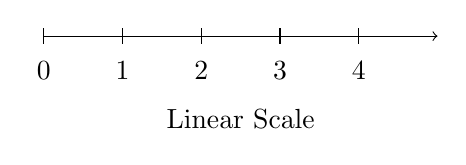
\begin{tikzpicture}
    \draw[->] (0,0) -- (5,0);
    \foreach \i in {0,1,2,3,4} {
    \draw (\i,0.1) -- (\i,-0.1);
    \node[below] at (\i, -0.2) {$\i$};
    }
    \node[below] at (2.5, -0.8) {Linear Scale};
\end{tikzpicture}
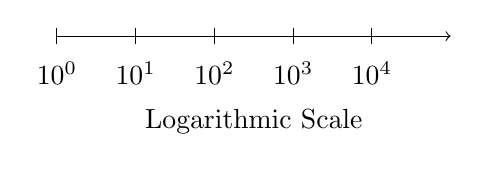
\begin{tikzpicture}
    \draw[->] (0,0) -- (5,0);
    \foreach \i in {0,1,2,3,4} {
    \draw (\i,0.1) -- (\i,-0.1);
    \node[below] at (\i, -0.2) {$10^{\i}$};
    }
    \node[below] at (2.5, -0.8) {Logarithmic Scale};
\end{tikzpicture}
\end{figure}

\item What is a logarithmic scale?
\item What is the difference between a linear scale and a logarithmic scale?

Slide rules were often used in the place of pocket calculators and without having to carry a table of logarithms.\\

\begin{figure}[h!]
\centering
\includegraphics[width=\linewidth]{slide rule drawing.jpeg}
    \caption*{Multiplication by Slide Rule (using powers of 2)}
\end{figure}

A slide rule consists of two logarithmic scales that can be slid against each other. Multiplication is done by aligning the start of the bottom scale to the multiplicand on the top scale, so the product becomes the number above the multiplier.\\

\begin{figure}[h!]
\centering
\includegraphics[width=\textwidth]{slide rule cropped.jpg}
\caption*{Slide Rule}
\end{figure}

 Prior to the 1980s, slide rules were indispensable tools for scientists, mathematicians, and engineers. These essential instruments played a pivotal role in the calculations behind every major engineering project and significant scientific advancement. Even as NASA made its initial foray into early computing, slide rules remained a constant companion for their engineers. In fact, it's remarkable to note that the remarkable achievement of sending humans to the moon was accomplished with slide rules, rather than the modern calculators of today.
 
\item What is a slide rule?
\item How were slide rules better than a table of logarithms?
\item How do you multiply using a slide rule?
\item How would you do division with a slide rule?

\subsection*{Antilogarithms}
As you have seen in the final step of the use of logarithms to simplify operations with large numbers, an antilogarithm reverses a logarithm. It is the number that was turned into a logarithm in the first place. Given the logarithm of an unknown number, how do you find the number? Usually finding the antilogarithm gives the solution to the problem.\\

Antilogarithm is usually abbreviated as antilog.\\

Say $\log{x}\approx0.4771$. The antilog is the number that 0.4771 is the log of.\\

The definition of a log is that if $n = b^e$, $\log_b{n}=e$, so $\log_{10}{x}\approx0.4771$ can be rearranged to become x\approx10^{0.4771}\approx3$. In other words, the antilog of 0.4771 is 3.\\

It is the same for a base other than 10, such as $\log_5{x}\approx0.6065$. This rearranges to become $x$ (the antilog) $\approx5^{0.6065}\approx2.6541$.\\

The antilogarithm can be calculated as a power, or looked up in reverse from a table of logarithms.\\

\item What is an antilogarithm?
\item How do you find the antilogarithm of a number?
\item If $\log_{10}x=2.1673$, then what is the antilog?
\item If $\log_{5}x=13.1326$, then what is the antilog?

\section*{Properties of Logarithms}

\begin{Large}
$$\log_a{1}=0$$
\end{Large}
\begin{center}
\text{(because }$n^0=0$
\end{center}
\begin{align*}
\text{also: }\ln{1}&=0\\
\text{and: }\log{1}&=0
\end{align*}

\begin{Large}
$$\log_a{a}=1$$
\end{Large}
\begin{center}
\text{(because }$n^1=n$\\
\end{center}

\begin{align*}
\text{also: }\ln{e}&=1\\
\text{and: }\log{10}&=1
\end{align*}

\begin{Large}
$$log_a{a^n}=n$$
\end{Large}
\begin{align*}
\text{also: }\ln{e^n}&=n\\
\text{and: }\log10^n&=n
\end{align*}

\begin{Large}
$$a^{log_b{n}}=n$$
\end{Large}
\begin{align*}
\text{also: }e^{\ln{x}}&=x\\
\text{and: }10^{\log{x}}&=x
\end{align*}

\item What is $\log1$?
\item What is $\log_{5}1$?
\item What is $\log_{2}1$?
\item What is $\ln{1}$?

\item What is $\log10$?
\item What is $\ln{e}$?
\item What is $\log_{5}5$?
\item What is $\log_{2}2$?

\item What is $\log_{5}5^2$?
\item What is $\log_{3}3^5$?
\item What is $\log10^3$?
\item What is $\ln{e^6}$?

\item What is $3^{\log_{5}4}$?
\item What is $8^{\log_{5}1}$?
\item What is $e^{\ln{7}}$?
\item What is $10^{\log9}$?

\section*{Log Rules}

\subsection*{Product Rule}
\begin{Large}
$$\log_b{A}+\log_b{B}=\log_b{AB}$$
\end{Large}

\begin{center}
\begin{tabular}{lll}
\text{proof:}&$\text{let }log_b{A}=x$            & $A = b^x$\\
             &$\text{let }\log_b{B}=y$           & $B = b^y$\\
             &                                   &\\
\text{so }   &$AB=b^x b^y=b^{x+y}$               &\\
             &$log_b{AB}=x+y=log_b{A}+log_b{B}$  &
\end{tabular}
\end{center}

\begin{align*}
\text{e.g. } \log_2{5}+log_2{4}
                         &=\log_2{(5\cdot4)}=\log_2{20}\\
                         &       \\
\text{e.g. given }\log{2}&=0.3010\\
\text{ and }      \log{3}&=0.4771\\
\text{ and }      \log{5}&=0.6990\\
\text{then }     \log{30}&=\log{(2\cdot3\cdot5)}\\
                         &=\log{2}+\log{3}+\log{5}=1.4771
\end{align*}

\item What is $\log_2{8} + \log_2{2}$?
\item What is $\log_3{9} + \log_3{27}$?
\item What is $\ln{e} + \ln{7}$?
\item If $\log_a{2} = 0.3010$ and $\log_a{3} = 0.4771$, find $\log_a{(2 \cdot 3)}$.
\item If $\log_b{4} = 1.3863$ and $\log_b{5} = 0.6989$, find $\log_b{(4 \cdot 5)}$.
\item If $\log_c{10} = 1$ and $\log_c{7} = 0.8451$, find $\log_c{(10 \cdot 7)}$.

\subsection*{Quotient Rule}
\begin{Large}
$$\log_b{A}-\log_b{B}=\log_b\frac{A}{B}$$
\end{Large}

\begin{center}
\begin{tabular}{ l l l }
\text{proof:}&\text{let }$\log_b{A}=x$ & $A = b^x$\\
             &\text{let }$\log_b{B}=y$ & $B = b^y$\\
             &                         &          \\
             &\text{so	}$\frac{A}{B}=\frac{b^x}{b^y}=b^{x-y}$&\\
             &$\log_b{\frac{A}{B}}=x-y=\log_b{A}-\log_b{B}$&
\end{tabular}
\end{center}

\begin{align*}
\text{e.g. }\log_2{20}+log_2{4}&
=\log_2{(\frac{20}{4})}=\log_2{5}\\
\cr
\text{e.g. given }\log{2}&=0.3010\\
\text{then }\log{50}&=\log{(\frac{100}{2})}\\
&=\log{100}-\log{2}
\text{  }(\log_{10}{100}=2)\\
&=2-0.3010=1.699
\end{align*}

\item What is $\log_3{27} - \log_3{9}$
\item What is $\log_4{64} - \log_4{8}$
\item What is $\log_2{16} - \log_2{4}$
\item What is $\log_5{125} - \log_5{5}$
\item If $\log_a{8} = 0.9031$ and $\log_a{2} = 0.3010$, find $\log_a{(8 / 2)}$.
\item If $\log_b{100} = 2$ and $\log_b{4} = 0.6021$, find $\log_b{(100 / 4)}$.

\subsection*{Power Rule}
\begin{Large}
$$log_a{x^n}=n\log_a{x}$$
\end{Large}

\begin{center}
\begin{tabular}{ l l l l }
\text{proof:}&\text{let }$m=\log_a{x}=x$         & $x = a^m$\\
             &\text{so	}$x^n=({a^m})^n=a^{mn}$ &\\
             & $\log{x^n}=mn=nm=n\log_a{x}$      &
\end{tabular}
\end{center}

\begin{align*}
\text{e.g. }\log{x^4}              &=4\log{x}\\
                                   &\\
\text{e.g. }\log_3{\frac{1}{3}}    &=log_3{1}-log_3{3}\\
                                   &=0-1=-1\\
                                   &\text{(}\log_a{1}=0\text{ and }\log_a{a}=1\text{)}\\
                                   &\\
\text{e.g. }\log{\sqrt{10}}        &=\log10^{\frac{1}{2}}\\
                                   &=\frac{1}{2}\log{10}\\
                                   &=\frac{1}{2}\cdot1=\frac{1}{2}
\end{align*}

\item What is $\log_2{(2^4)}$?
\item What is $\log_5{(5^2)}$?
\item What is $\log_3{(3^2)} + \log_3{(3^4)}$?
\item What is $\log{(10^3)} - \log{(10^2)}$?
\item What is $\ln{(e^5)} + \ln{(e^3)}$?
\item What is $\log_2{(2^7)} - \log_2{(2^5)}$?
\item What is $2\log_2{3}$ as a single logarithm?
\item What is $4\log_{10}{7}$ as a single logarithm?
\item What is $-2\ln{(e^2)}$ as a single logarithm?
\item What is $\log_4{(4^{3/2})}$?
\item What is $\log_{2}{(2^{7/2})} - \log_{2}{(2^{3/2})}$?
\item What is $\ln{(e^{1/3})} + \ln{(e^{5/3})}$?

\subsection*{Root Rule}
\begin{Large}
$$\log_a{(\sqrt[n]{x})}=\frac{\log_a{x}}{n}$$
\end{Large}
\\

\begin{align*}
\text{e.g.}
\log_2{\sqrt{8}}&=\frac{\log_2{8}}{2}=\frac{3}{2}\\
\\
\text{e.g.}
\log_3{\sqrt{9}}&=\frac{\log_3{9}}{2}=\frac{2}{2}=1
\end{align*}

\item What is $\log_2{(\sqrt[3]{64})}$?
\item What is $\log{(\sqrt[4]{10,000})}$?
\item What is $\ln{(\sqrt[5]{e^5})}$?
\item What is $\log_3{(\sqrt[2]{81})}$?
\item What is $\log_{9}{(\sqrt[2]{9^{10}})}$?
\item What is $\ln{(\sqrt[4]{e^8})}$?
\item What is $\frac{1}{3}\log_2{8}$?
\item What is $\frac{1}{4}\log_{10}{10,000}$?
\item What is $\frac{1}{5}\ln{(e^{10})}$?
\item What is $\log_{11}{(\sqrt[3]{11^{9}})}$?
\item What is $\log_{2}{(\sqrt[5]{2^{15}})}$?
\item What is $\ln{(\sqrt[7]{e^{21}})}$?

\subsection*{Change of Base Law}

It is unusual to have to find a log for a number with a base other than 10 or $e$, but there is a formula that can be used:

\begin{Large}
$$\log_a{n}=\frac{\log_b{n}}{\log_b{a}}$$
\end{Large}

\begin{align*}

\text{for base 10}
\log_a{n}&=\frac{\log_{10}{n}}{\log_{10}{a}}=\frac{\log{n}}{\log{a}}\\

\text{for base e}
\log_a{n}&=\frac{\log_{e}{n}}{\log_{e}{a}}=\frac{\log{n}}{\log{a}}
\end{align*}

\onehalfspacing

\begin{center}
\begin{tabular}{llll}
proof: & $\log_a{n}                 &= mn = a^m$      & (by definition)\\
       &$\log_b{n}                  &= \log_b{a^m}$  & (taking log of both sides)\\
       &$\log_b{n}                  &= m \log_b{a}$   & (using power rule)\\
       &$\frac{\log_b{n}}{\log_b{a}}&= m = \log_a{n}$& (rearranging)
\end{tabular}
\end{center}

\singlespacing

\begin{center}
\begin{equation*}
\begin{split}
\text{e.g. }\log_4{40}        &=\frac{\log{40}}{\log{4}}\\
                              &=\frac{16.0206}{0.60206}=2.661\\\\
\text{e.g. }\log_2{5}+log_3{7}&=(\frac{\log{5}}{\log{2}})+(\frac{\log{7}}{\log{3}})\\
                              &=4.0932\\\\
\text{e.g. }\log{x}+3\log{y}-4\log{z}&=\log{x}+\log{y^3}-\log{z^4}\\
                              &=\log\frac{x{y^3}}{z^4}\\\\
\text{e.g. }2+4\log_3{x}      &=\log_3{9}+\log_3{x^4}\\
                              &=\log_3{9x^4}\\
&\text{(express 2 as a log with base 3: }\\
&$2 = 2\log_3{3}=\log_3{3^2}=\log_3{9})$
\end{split}
\end{equation*}
\end{center}

\item What is $\log_6{36}$ with a base of 2?
\item What is $\log{1000}$ with a base of 5?
\item What is $\ln{100}$ with a base of 4?
\item What is $\log_7{49}$ with a base of 3?
\item What is $\log_3{7} + \log_2{9}$?
\item What is $\log_{4}{16} - \log_{2}{64}$?
\item What is $\log{100} + \log_{5}{25}$?
\item What is $\ln{e^3} - \ln{e^2}$?
\item What is $\log_{2}{16} + \log_{3}{9}$ with a base of 4?
\item What is $\log_{5}{125} - \log{100}$ with a base of 2?
\item What is $\log_{5}{25} + \log_{5}{5}$ with a base of 10?
\item What is $\ln{e^5} + \log_{2}{2^3}$ with a base of 10?

\section*{Logarithmic Equations}

\subsection*{Using the Definition of a Logarithm}

\begin{center}
\begin{tabular}{llll}
\text{e.g. }&$\log_10{x}=2$ & $\longrightarrow x=10^2$ & $\longrightarrow x=100$\\
\text{e.g. }&$\log_x{25}=2$ & $\longrightarrow25=x^2$ & $\longrightarrow x=\pm5=5$\\
\text{e.g. }&$\log_x{22}=2.1$ & $\longrightarrow22=x^{2.1}$ & $\longrightarrow x=\sqrt[2.1]{22}=4.358$\\
\text{e.g. }&$\log_4{5}=x$ & $\longrightarrow\frac{\log{5}}{\log{4}}=1.161$\\
\end{tabular}
\end{center}

\item Solve for $x$: $\log_3{x} = 4$
\item Solve for $x$: $\log{x} = 1$
\item Solve for $x$: $\log_2{x} = 3$
\item Solve for $x$: $\ln{x} = 0$
\item Solve for $x$: $\log_{4}{x} = 2$
\item Solve for $x$: $\log_7{x} = 1.5$
\item Solve for $x$: $\ln{e}{x} = -2$
\item Solve for $x$: $\log_{3}{x} = 2.5$
\item Solve for $x$: $\log{x} = 2.5$
\item Solve for $x$: $\log_2{x} = 2.5$
\item Solve for $x$: $\ln{x} = 2.5$
\item Solve for $x$: $\ln{x} = 0.5$

\subsection*{Using Equivalence}
(equivalence: if $log_b{x}=log_b{y}$ then $x=y$.)
\begin{align*}
\text{e.g. }\log{x}+\log{5}&=\log{20}\\
\log{5x}&=\log{20}\text{ (product rule)}\\
5x&=20\\
x&=4
\end{align*}

\item Solve for $x$: $\log{x} + \log{3} = \log{9}$.
\item Solve for $x$: $\log{2x} = \log{16}$.
\item Solve for $x$: $\log{4x} + \log{2} = \log{32}$.
\item Solve for $x$: $\log{x} - \log{4} = \log{2}$.
\item Solve for $x$: $\log{x} + \log{5} = \log{125}$.
\item Solve for $x$: $\log{3x} = \log{27}$.
\item Solve for $x$: $\log{x} + \log{7} = \log{49}$.
\item Solve for $x$: $\log{8x} + \log{2} = \log{128}$.
\item Solve for $x$: $\log{3x} - \log{9} = \log{1}$.
\item Solve for $x$: $\log{x} + \log{11} = \log{121}$.
\item Solve for $x$: $\log{12x} + \log{2} = \log{288}$.
\item Solve for $x$: $\log{2x} - \log{16} = \log{8}$.

\subsection*{Grouping Log Terms to one side}

(Rearranging to get log terms on on side\\ and numbers on the other)
\begin{align*}
\text{e.g. }\log_4{(2x+4)}-2&=\log_4{3}\\
\log_4{(2x+4)}-\log_4{3}&=2\\
\log_4{\frac{2x+4}{3}}&=2\\
\frac{2x+4}{3}&=4^2\\
\frac{2x+4}{3}&=16\\
2x+4&=48\\
2x&=44\\
x&=22
\end{align*}

\item Solve for $x$: $\log_3{(3x+6)}-2 = \log_3{9}$.
\item Solve for $x$: $\log_2{(4x+8)} - \log_2{2} = 3$.
\item Solve for $x$: $\log_5{(5x+10)} - \log_5{5} = 1$.
\item Solve for $x$: $\log{(10x+20)} - \log{2} = 4$.
\item Solve for $x$: $\ln{(ex+2e)} - \ln{e} = 2$.

\subsection*{Replacing a Number\\ with the Equivalent Log}
\begin{align*}
\text{e.g. }\log_4{(2x+4)}-2&=\log_4{3}\\
\log_4{(2x+4)}-\log_4{16}&=\log_4{3}\\
\log_4{(2x+4)}-\log_4{4^2}&=\log_4{3}\\
\log_4\frac{2x+4}{16}&=log_4{3}\\
\frac{2x+4}{16}&=3\\
2x+4&=48\\
2x&=44\\
x&=22
\end{align*}

\item Solve for $x$: $\log_2{(x+4)} = 3$.
\item Solve for $x$: $\log{(2x+6)} = \log{100}$.
\item Solve for $x$: $\log_5{(3x+9)} = \log_5{125}$.
\item Solve for $x$: $\ln{(4x+8)} = \ln{e^3}$.
\item Solve for $x$: $\log_3{(5x+10)} = \log_3{3^2}$.

\section*{Exponential Equations}

Exponential equations deal with rates of growth and decay. They take their name from the fact that they contain terms with exponents. Exponential equations were first used in calculating compound interest and in population growth. They have many uses. Logarithms provide a method to solve exponential equations that would be difficult or impractical to solve algebraically.\\

Here are some examples from the field of finance:\\

How long will it take investor who deposits \$20,000 compounding at 5 \% p.a. to increase this amount to \$30,000?

Compound Interest Formula: $A=P(1+i)^n$

- \(A\) is the final amount (in this case, $\$30,000$).

- \(P\) is the principal amount (initial investment, in this case, $\$20,000$).

- \(i\) is the annual interest rate (in this case, $5\%$ or \(0.05\) as a decimal).

- \(n\) is the number of years (which we need to find).
\begin{align*}
30,000&=20,000(1.05)^n\\
\frac{30,000}{20,000}&=1.05^n\\
1.5&=1.05^n\\
\log{1.5}&=\log{1.05^n}\\
\log{1.5}&=n\log{1.05}\\
\frac{\log{1.5}}{\log{1.05}}&=n\\
\frac{0.1761}{0.2119}&\approx8.3\text{ years}\\
[1.05^{8.31}&\approx1.5\ \checkmark ]
\end{align*}

\item How long will it take for an investment of \$$10,000$ to grow to \$$15,000$ when compounded annually at a rate of $4\%$?

\[\$15,000 = \$10,000(1 + 0.04)^n\]
\[1.5 = (1.04)^n\]
\[\ln(1.5) = \ln(1.04^n)\]
\[\ln(1.5) = n \cdot \ln(1.04)\]
\[n = \frac{\ln(1.5)}{\ln(1.04)}\]
\[n \approx \frac{0.4055}{0.0392} \approx 10.34\text{ years}]

\item An individual invests \$$25,000$ in a savings account, and the account grows to \$$30,000$ after a certain number of years with an annual interest rate of $3\%$. Find the number of years it took to reach this amount.
\item If \$$5,000$ is invested at a $6\%$ annual interest rate, how many years will it take for the investment to double in value?
\item A deposit of \$$8,000$ earns $7\%$ annual interest. Determine the number of years it takes for the deposit to reach \$$10,000$.
\item If an investment of \$$50,000$ grows to \$$60,000$ with a $5\%$ annual interest rate, how many years did it take to achieve this growth?\\

Here is an example from the field of physics involving radioactive decay:

The decay of a radioactive substance over time can be modeled using the exponential decay equation:

\begin{equation*}
N(t) = N_0 \times e^{-\lambda t}
\end{equation*}
Where:
\begin{align*}
N(t) & : \text{Remaining quantity of radioactive substance at time } t \\
N_0 & : \text{Initial quantity of radioactive substance} \\
\lambda & : \text{Decay constant} \\
t & : \text{Time elapsed}
\end{align*}

Suppose we have an initial quantity of a radioactive substance, and we want to find the time it takes for the substance to decay to a certain fraction of its initial amount. Let's say we want to find the time when the remaining quantity is $\frac{N_0}{2}$.

Using the exponential decay equation, we have:

\[\frac{N_0}{2} = N_0 \times e^{-\lambda t}\]

Dividing both sides by $N_0$ and taking the natural logarithm (base $e$) of both sides:

\begin{align*}
\ln{\left(\frac{N_0}{2}\right)} &= \ln{(N_0 \times e^{-\lambda t})} \\
\ln{\left(\frac{1}{2}\right)} &= \ln{(e^{-\lambda t})} \\
\ln{\left(\frac{1}{2}\right)} &= -\lambda t \ln{e} \\
\ln{\left(\frac{1}{2}\right)} &= -\lambda t \\
t &= -\frac{\ln{\left(\frac{1}{2}\right)}}{\lambda}
\end{align*}

This formula allows us to calculate the time it takes for any radioactive substance to decay to half of its initial amount, given its decay constant.

Here is another worked example:

Suppose a sample of a radioactive substance has an initial quantity of $N_0 = 1000$ grams and a decay constant $\lambda = 0.05$ per year. We want to find the time it takes for the substance to decay to $250$ grams.

Using the exponential decay equation:

\[N(t) = N_0 \times e^{-\lambda t}\]

Substituting the known values:

\[250 = 1000 \times e^{-0.05t}\]
\[\frac{250}{1000} = \frac{1}{4} = e^{-0.05t}\]
\[\ln{\left(\frac{1}{4}\right)} = \ln{(e^{-0.05t})}\]
\[\ln{\left(\frac{1}{4}\right)} = -0.05t \ln{e}\]
\[(ln{e} = 1)\]
\[\ln{\left(\frac{1}{4}\right)} = -0.05t\]
\[t = \frac{\ln{\left(\frac{1}{4}\right)}}{-0.05} \approx 27.73\text{ years}\]

1. A radioactive substance initially has a quantity of $N_0 = 200$ grams and a decay constant $\lambda = 0.02$ per year. Calculate the time it takes for the substance to decay to $50$ grams.

2. In a laboratory experiment, a radioactive material with an initial quantity of $N_0 = 5000$ grams is observed to decay to $2500$ grams in a certain time. Find the decay constant $\lambda$ for this substance.

3. A sample of a radioactive element with $N_0 = 300$ grams and $\lambda = 0.03$ decays over time. Calculate the time it takes for the substance to decay to $75$ grams.

4. The half-life of a radioactive substance is 10 years. Find the decay constant $\lambda$ for this substance.

\end{enumerate}

\end{document}
